\documentclass[../xdudla00-porting-Tang-to-Open-WRT.tex]{subfiles}

\begin{document}

\chapter{Encryption}\label{encryption}


We may not realize this, but we use encryption every day.
The purpose of encryption is to keep us safe when we are browsing the internet or just storing our sensitive information on digital media. 
In general encryption is used to secure our data, whether transmitted around the internet or stored on our hard drives, from being compromised.
The encryption protects us from many threats.

It protects us from identity theft. 
Our personal information stored all over governmental authorities are secured with it.
Encryption care for not revealing sensitive information about ourselves, to protect our financial details, passwords and so on. 
Mainly when we bank online from being scammed.

It look after our conversation privacy. 
To be more specific our cell phone conversations from eavesdroppers and our online chatting with acquaintances or colleagues. 
It also allows attorneys to communicate privately with their clients and it aims to secure communication between investigation bureaus to exchange sensitive information about lawbreakers.

If we encrypt our laptop or desktop computer's hard drive the encryption protects our data in case the computer or hard drive would be stolen.

\section{Security and encryption}

Security is not a binary; it is a sliding scale of risk management \cite{devconf}.
People are used to mark things, for example good and bad, expensive, and cheap.
But we know that it may differ on person.
For example, there is no such thing as line or sign which tells us, this part of town is secure, and this is not. 
The way we reason about security is that we enter into this environment and we begin to study it and decide whether it is secure or not. 
Especially at enterprise sector. 

Encrypting does not actually have to be enough to tag data and/or infrastructure secure.
Companies define their own security strategies which may include encryption or not at all. 
It all relies on company's needs or will to take risks in idea of getting high gain from them.
In any case, the encryption is definitely a demanding element of security.

According to 2016 Global Encryption Trends Study, independently conducted by the Ponemon Institute\cite{Thales}, the enterprise-wide encryption increased from 15 to 38 percent.
Also the ratio of companies with no encryption strategy at all decreased from 37 to 15 percent. 
More than 50 percent companies are using extensively deployed encryption technologies to encrypt mostly databases, infrastructure and laptop hard drives. 

\section{Hard drive encryption}

It all starts, as mentioned, with desire to keep our data to ourselves and as a secret to the others.
More often than not, these secrets are stored on our hard drives.
Then lets take a look on how the encryption is typically done.

To protect our secrets we usually encrypt these data by using an encryption key - see Figure \ref{fig:encdata}.
However, our secret data might grow in size, and it is time and resource consuming to decrypt and encrypt the secret every time encryption key changes or it is compromised.
Because of that, we wrap encrypted data in the key encryption key. 
This key is actually user typed pass phrase and the system prompts this key from us when booting or simply when it wants to access our hard drive.

\begin{figure}[h]
    \centering
    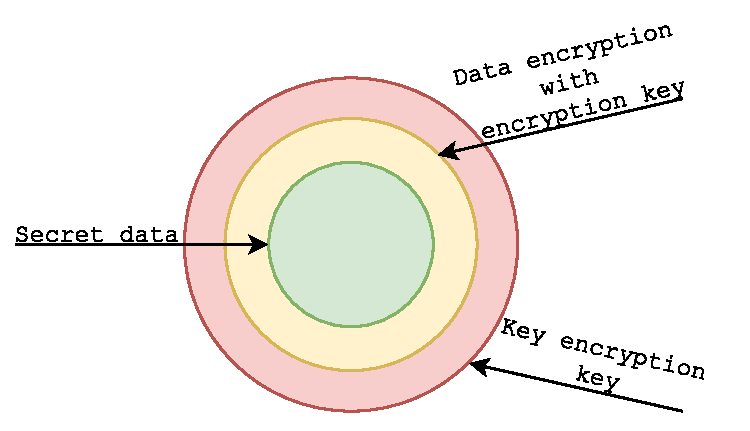
\includegraphics[scale=0.7]{figures/HowWeEncryptData.pdf}
    \caption{How we encrypt data}
    \label{fig:encdata}
\end{figure}

So, changing the key encryption key does not affect encrypted data.
We can change it whenever we desire to, and redistribute the new key to all users or services who are supposed to access these data.

To automatize this procedure, we could generate cryptographically stronger key encryption key than user provided password.
Then, we store this random key on a remote system, from where we can get or change it later.
This is basically how the key escrow \ref{escrow} model works.

For people is common to have a password protected system.
Imagine you come home in a mood to enjoy your time and your system asks for password, not once, but twice.
This might be the reason why most of us do not use encryption, even when we know it will protect our data.
Tang \ref{tang} server is solution for this, since we want to automatize things.

\subsection{LUKS}
\todo{LUKS HEADER IMAGE}


\subsection{Bit Locker}

\end{document}
